\documentclass[portrait,final,a0paper]{baposter}
%\documentclass[a4shrink,portrait,final]{baposter}
% Usa a4shrink for an a4 sized paper.

\tracingstats=2

\usepackage{calc}
\usepackage{graphicx}
\usepackage{amsmath}
\usepackage{amssymb}
\usepackage{relsize}
\usepackage{multirow}
\usepackage{bm}

\usepackage{multicol}

\usepackage{tikz}
\usetikzlibrary{matrix,arrows}
% \usepackage{pgfbaselayers}
% \pgfdeclarelayer{background}
% \pgfdeclarelayer{foreground}
% \pgfsetlayers{background,main,foreground}

\usepackage{times}
\usepackage{helvet}
%\usepackage{bookman}
\usepackage{palatino}

\newcommand{\captionfont}{\footnotesize}

%%%%%%% WJD: MY COMMANDS %%%%%%%%%%%%%
\newcommand{\Hawaii}{Hawai\kern.05em`\kern.05em\relax i}
\newcommand{\Manoa}{M\=anoa}
\newcommand{\bA}{\ensuremath{\mathbf{A}}}
\newcommand{\bCon}{\ensuremath{\mathbf{Con}}}
\newcommand{\<}{\ensuremath{\langle}}
\renewcommand{\>}{\ensuremath{\rangle}}
\newcommand{\algA}{\ensuremath{\< A; F\>}}

\selectcolormodel{cmyk}

\graphicspath{{baposter/images/}}

%%%%%%%%%%%%%%%%%%%%%%%%%%%%%%%%%%%%%%%%%%%%%%%%%%%%%%%%%%%%%%%%%%%%%%%%%%%%%%%%
%%%% Some math symbols used in the text
%%%%%%%%%%%%%%%%%%%%%%%%%%%%%%%%%%%%%%%%%%%%%%%%%%%%%%%%%%%%%%%%%%%%%%%%%%%%%%%%
% Format 
\newcommand{\Matrix}[1]{\begin{bmatrix} #1 \end{bmatrix}}
\newcommand{\Vector}[1]{\Matrix{#1}}
\newcommand*{\SET}[1]  {\ensuremath{\mathcal{#1}}}
\newcommand*{\MAT}[1]  {\ensuremath{\mathbf{#1}}}
\newcommand*{\VEC}[1]  {\ensuremath{\bm{#1}}}
\newcommand*{\CONST}[1]{\ensuremath{\mathit{#1}}}
\newcommand*{\norm}[1]{\mathopen\| #1 \mathclose\|}% use instead of $\|x\|$
\newcommand*{\abs}[1]{\mathopen| #1 \mathclose|}% use instead of $\|x\|$
\newcommand*{\absLR}[1]{\left| #1 \right|}% use instead of $\|x\|$

\def\norm#1{\mathopen\| #1 \mathclose\|}% use instead of $\|x\|$
\newcommand{\normLR}[1]{\left\| #1 \right\|}% use instead of $\|x\|$

%%%%%%%%%%%%%%%%%%%%%%%%%%%%%%%%%%%%%%%%%%%%%%%%%%%%%%%%%%%%%%%%%%%%%%%%%%%%%%%%
% Multicol Settings
%%%%%%%%%%%%%%%%%%%%%%%%%%%%%%%%%%%%%%%%%%%%%%%%%%%%%%%%%%%%%%%%%%%%%%%%%%%%%%%%
\setlength{\columnsep}{0.7em}
\setlength{\columnseprule}{0mm}


%%%%%%%%%%%%%%%%%%%%%%%%%%%%%%%%%%%%%%%%%%%%%%%%%%%%%%%%%%%%%%%%%%%%%%%%%%%%%%%%
% Save space in lists. Use this after the opening of the list
%%%%%%%%%%%%%%%%%%%%%%%%%%%%%%%%%%%%%%%%%%%%%%%%%%%%%%%%%%%%%%%%%%%%%%%%%%%%%%%%
\newcommand{\compresslist}{%
\setlength{\itemsep}{1pt}%
\setlength{\parskip}{0pt}%
\setlength{\parsep}{0pt}%
}


%%%%%%%%%%%%%%%%%%%%%%%%%%%%%%%%%%%%%%%%%%%%%%%%%%%%%%%%%%%%%%%%%%%%%%%%%%%%%%
%%% Begin of Document
%%%%%%%%%%%%%%%%%%%%%%%%%%%%%%%%%%%%%%%%%%%%%%%%%%%%%%%%%%%%%%%%%%%%%%%%%%%%%%

\begin{document}

%%%%%%%%%%%%%%%%%%%%%%%%%%%%%%%%%%%%%%%%%%%%%%%%%%%%%%%%%%%%%%%%%%%%%%%%%%%%%%
%%% Here starts the poster
%%%---------------------------------------------------------------------------
%%% Format it to your taste with the options
%%%%%%%%%%%%%%%%%%%%%%%%%%%%%%%%%%%%%%%%%%%%%%%%%%%%%%%%%%%%%%%%%%%%%%%%%%%%%%
% Define some colors
\definecolor{silver}{cmyk}{0,0,0,0.3}
\definecolor{yellow}{cmyk}{0,0,0.9,0.0}
\definecolor{reddishyellow}{cmyk}{0,0.22,1.0,0.0}
\definecolor{black}{cmyk}{0,0,0.0,1.0}
\definecolor{darkYellow}{cmyk}{0,0,1.0,0.5}
\definecolor{darkSilver}{cmyk}{0,0,0,0.1}
\definecolor{OliveGreen}{cmyk}{0.64,0,0.95,0.40} % PANTONE 582

\definecolor{lightyellow}{cmyk}{0,0,0.3,0.0}
\definecolor{lighteryellow}{cmyk}{0,0,0.1,0.0}
\definecolor{lighteryellow}{cmyk}{0,0,0.1,0.0}
\definecolor{lightestyellow}{cmyk}{0,0,0.05,0.0}

% "Crayola" color definitions
% originally due to Tomas Rokick for his dvips definitions.
\definecolor{GreenYellow}{cmyk}{0.15,0,0.69,0} % PANTONE 388
\definecolor{Yellow}{cmyk}{0,0,1.,0} % PANTONE YELLOW
\definecolor{Goldenrod}{cmyk}{0,0.10,0.84,0} % PANTONE 109
\definecolor{Dandelion}{cmyk}{0,0.29,0.84,0} % PANTONE 123
\definecolor{Apricot}{cmyk}{0,0.32,0.52,0} % PANTONE 1565
\definecolor{Peach}{cmyk}{0,0.50,0.70,0} % PANTONE 164
\definecolor{Melon}{cmyk}{0,0.46,0.50,0} % PANTONE 177
\definecolor{YellowOrange}{cmyk}{0,0.42,1.,0} % PANTONE 130
\definecolor{Orange}{cmyk}{0,0.61,0.87,0} % PANTONE ORANGE-021
\definecolor{BurntOrange}{cmyk}{0,0.51,1.,0} % PANTONE 388
\definecolor{Bittersweet}{cmyk}{0,0.75,1.,0.24} % PANTONE 167
\definecolor{RedOrange}{cmyk}{0,0.77,0.87,0} % PANTONE 179
\definecolor{Mahogany}{cmyk}{0,0.85,0.87,0.35} % PANTONE 484
\definecolor{Maroon}{cmyk}{0,0.87,0.68,0.32} % PANTONE 201
\definecolor{BrickRed}{cmyk}{0,0.89,0.94,0.28} % PANTONE 1805
\definecolor{Red}{cmyk}{0,1.,1.,0} % PANTONE RED
\definecolor{OrangeRed}{cmyk}{0,1.,0.50,0} % No PANTONE,match
\definecolor{RubineRed}{cmyk}{0,1.,0.13,0} % PANTONE RUBINE-RED
\definecolor{WildStrawberry}{cmyk}{0,0.96,0.39,0} % PANTONE 206
\definecolor{Salmon}{cmyk}{0,0.53,0.38,0} % PANTONE 183
\definecolor{CarnationPink}{cmyk}{0,0.63,0,0} % PANTONE 218
\definecolor{Magenta}{cmyk}{0,1.,0,0} % PANTONE PROCESS-MAGENTA
\definecolor{VioletRed}{cmyk}{0,0.81,0,0} % PANTONE 219
\definecolor{Rhodamine}{cmyk}{0,0.82,0,0} % PANTONE RHODAMINE-RED
\definecolor{Mulberry}{cmyk}{0.34,0.90,0,0.02} % PANTONE 241
\definecolor{RedViolet}{cmyk}{0.07,0.90,0,0.34} % PANTONE 234
\definecolor{Fuchsia}{cmyk}{0.47,0.91,0,0.08} % PANTONE 248
\definecolor{Lavender}{cmyk}{0,0.48,0,0} % PANTONE 223
\definecolor{Thistle}{cmyk}{0.12,0.59,0,0} % PANTONE 245
\definecolor{Orchid}{cmyk}{0.32,0.64,0,0} % PANTONE 252
\definecolor{DarkOrchid}{cmyk}{0.40,0.80,0.20,0} %  No PANTONE match
\definecolor{Purple}{cmyk}{0.45,0.86,0,0} % PANTONE PURPLE
\definecolor{Plum}{cmyk}{0.50,1.,0,0} % PANTONE 518
\definecolor{Violet}{cmyk}{0.79,0.88,0,0} % PANTONE VIOLET
\definecolor{RoyalPurple}{cmyk}{0.75,0.90,0,0} % PANTONE 267
\definecolor{BlueViolet}{cmyk}{0.86,0.91,0,0.04} % PANTONE 2755
\definecolor{Periwinkle}{cmyk}{0.57,0.55,0,0} % PANTONE 2715
\definecolor{CadetBlue}{cmyk}{0.62,0.57,0.23,0} % PANTONE (534+535)
\definecolor{CornflowerBlue}{cmyk}{0.65,0.13,0,0} % PANTONE 292
\definecolor{MidnightBlue}{cmyk}{0.98,0.13,0,0.43} % PANTONE 302
\definecolor{NavyBlue}{cmyk}{0.94,0.54,0,0} % PANTONE 293
\definecolor{RoyalBlue}{cmyk}{1.,0.50,0,0} % No PANTONE match
\definecolor{Blue}{cmyk}{1.,1.,0,0} % PANTONE BLUE-072
\definecolor{Cerulean}{cmyk}{0.94,0.11,0,0} % PANTONE 3005
\definecolor{Cyan}{cmyk}{1.,0,0,0} % PANTONE PROCESS-CYAN
\definecolor{ProcessBlue}{cmyk}{0.96,0,0,0} % PANTONE PROCESS-BLUE
\definecolor{SkyBlue}{cmyk}{0.62,0,0.12,0} % PANTONE 2985
\definecolor{Turquoise}{cmyk}{0.85,0,0.20,0} % PANTONE (312+313)
\definecolor{TealBlue}{cmyk}{0.86,0,0.34,0.02} % PANTONE 3145
\definecolor{Aquamarine}{cmyk}{0.82,0,0.30,0} % PANTONE 3135
\definecolor{BlueGreen}{cmyk}{0.85,0,0.33,0} % PANTONE 320
\definecolor{Emerald}{cmyk}{1.,0,0.50,0} % No PANTONE match
\definecolor{JungleGreen}{cmyk}{0.99,0,0.52,0} % PANTONE 328
\definecolor{SeaGreen}{cmyk}{0.69,0,0.50,0} % PANTONE 3268
\definecolor{Green}{cmyk}{1.,0,1.,0} % PANTONE GREEN
\definecolor{ForestGreen}{cmyk}{0.91,0,0.88,0.12} % PANTONE 349
\definecolor{PineGreen}{cmyk}{0.92,0,0.59,0.25} % PANTONE 323
\definecolor{LimeGreen}{cmyk}{0.50,0,1.,0} % No PANTONE match
\definecolor{YellowGreen}{cmyk}{0.44,0,0.74,0} % PANTONE 375
\definecolor{SpringGreen}{cmyk}{0.26,0,0.76,0} % PANTONE 381
\definecolor{OliveGreen}{cmyk}{0.64,0,0.95,0.40} % PANTONE 582
\definecolor{RawSienna}{cmyk}{0,0.72,1.,0.45} % PANTONE 154
\definecolor{Sepia}{cmyk}{0,0.83,1.,0.70} % PANTONE 161
\definecolor{Brown}{cmyk}{0,0.81,1.,0.60} % PANTONE 1615
\definecolor{Tan}{cmyk}{0.14,0.42,0.56,0} % No PANTONE match
\definecolor{Gray}{cmyk}{0,0,0,0.50} % PANTONE COOL-GRAY-8
\definecolor{Black}{cmyk}{0,0,0,1.} % PANTONE PROCESS-BLACK
\definecolor{White}{cmyk}{0,0,0,0} % No PANTONE match

%%
\typeout{Poster Starts}
\background{
  \begin{tikzpicture}[remember picture,overlay]%
    \draw (current page.north west)+(-2em,2em) node[anchor=north west] {\includegraphics[height=1.1\textheight]{silhouettes_background}};
  \end{tikzpicture}%
}

\newlength{\leftimgwidth}
\begin{poster}%
  % Poster Options
  {
  % Show grid to help with alignment
  grid=no,
  % Column spacing
  colspacing=1em,
  % Color style
%  bgColorOne=lighteryellow,
  bgColorOne=white,
%  bgColorTwo=lightestyellow,
  bgColorTwo=white,
 borderColor=reddishyellow,
%  borderColor=yellow,
%  borderColor=Cerulean,
%  borderColor=Dandelion,
%  borderColor=BurntOrange,
%  headerColorOne=yellow,
  headerColorOne=OliveGreen,
%  headerColorTwo=reddishyellow,
%  headerColorTwo=TealBlue,
  headerFontColor=white,
  boxColorOne=lighteryellow,
  boxColorTwo=lighteryellow,
  % Format of textbox
  textborder=roundedleft,
%  textborder=rectangle,
  % Format of text header
  eyecatcher=no,
  headerborder=open,
  headerheight=0.08\textheight,
  headershape=roundedright,
  headershade=plain,
  headerfont=\Large\textsf, %Sans Serif
  boxshade=plain,
%  background=shade-tb,
  background=plain,
  linewidth=2pt
  }
  % Eye Catcher
  {\includegraphics[width=10em]{D1077}} % No eye catcher for this poster. (eyecatcher=no above). If an eye catcher is present, the title is centered between eye-catcher and logo.
  % Title
  {\sf %Sans Serif
  %\bf% Serif
  An Open Question About Finite Algebras
    \vspace{.3em}}
  % Authors
  {\sf %Sans Serif
  % Serif
    William DeMeo
    \vspace{1em} {\small \mbox{<}demeo@hawaii.edu\mbox{>}}
\hfill
 {\it University of \Hawaii\ at \Manoa}

  }
  % University logo
  {% The makebox allows the title to flow into the logo, this is a hack because of the L shaped logo.
    \makebox[8em][r]{%
      \begin{minipage}{16em}
        \hfill
        \includegraphics[height=2.3em]{Zapfino}
        \includegraphics[height=7.0em]{uh_logo}
      \end{minipage}
    }
  }

  \tikzstyle{light shaded}=[top color=baposterBGtwo!30!white,bottom color=baposterBGone!30!white,shading=axis,shading angle=30]

  % Width of left inset image
     \setlength{\leftimgwidth}{0.78em+8.0em}

%%%%%%%%%%%%%%%%%%%%%%%%%%%%%%%%%%%%%%%%%%%%%%%%%%%%%%%%%%%%%%%%%%%%%%%%%%%%%%
%%% Now define the boxes that make up the poster
%%%---------------------------------------------------------------------------
%%% Each box has a name and can be placed absolutely or relatively.
%%% The only inconvenience is that you can only specify a relative position 
%%% towards an already declared box. So if you have a box attached to the 
%%% bottom, one to the top and a third one which should be in between, you 
%%% have to specify the top and bottom boxes before you specify the middle 
%%% box.
%%%%%%%%%%%%%%%%%%%%%%%%%%%%%%%%%%%%%%%%%%%%%%%%%%%%%%%%%%%%%%%%%%%%%%%%%%%%%%
    %
    % A coloured circle useful as a bullet with an adjustably strong filling
    \newcommand{\colouredcircle}[1]{%
      \tikz{\useasboundingbox (-0.2em,-0.32em) rectangle(0.2em,0.32em); \draw[draw=black,fill=baposterBGone!80!black!#1!white,line width=0.03em] (0,0) circle(0.18em);}}

%%%%%%%%%%%%%%%%%%%%%%%%%%%%%%%%%%%%%%%%%%%%%%%%%%%%%%%%%%%%%%%%%%%%%%%%%%%%%%
  \headerbox{The Problem}{name=problem,column=0,row=0}{
%%%%%%%%%%%%%%%%%%%%%%%%%%%%%%%%%%%%%%%%%%%%%%%%%%%%%%%%%%%%%%%%%%%%%%%%%%%%%%
   {}A {\bf finite algebra} is an utterly fundamental object in mathematics.  The shape
   of an algebra's {\bf \mbox{congruence lattice}} gives us vital information about
   the algebra.  
  \vspace{0.3em}

   However, we still don't know whether there are any restrictions on
   the possible shapes of congruence lattices.  Mathematicians have been on a
   quest for over 50 years to either find such restrictions or prove that none exist.

  \vspace{0.3em}
  }
%%%%%%%%%%%%%%%%%%%%%%%%%%%%%%%%%%%%%%%%%%%%%%%%%%%%%%%%%%%%%%%%%%%%%%%%%%%%%%
  \headerbox{Contribution}{name=contribution,column=0,below=problem}{
%%%%%%%%%%%%%%%%%%%%%%%%%%%%%%%%%%%%%%%%%%%%%%%%%%%%%%%%%%%%%%%%%%%%%%%%%%%%%%
   {}We have identified large classes of lattices which occur as congruence
   lattices of finite algebras, and have found ways to build new
   ``representable'' lattices out of old ones.  Thus, we have made significant progress 
   toward a possible answer to this basic question:
  \vspace{0.3em}

   ``Is there a finite lattice which cannot be the congruence lattice of a
   finite algebra?''   
  \vspace{0.3em}

 }

%%%%%%%%%%%%%%%%%%%%%%%%%%%%%%%%%%%%%%%%%%%%%%%%%%%%%%%%%%%%%%%%%%%%%%%%%%%%%%
  \headerbox{What is an algebra?}{name=algebra,column=0,below=contribution}{
%%%%%%%%%%%%%%%%%%%%%%%%%%%%%%%%%%%%%%%%%%%%%%%%%%%%%%%%%%%%%%%%%%%%%%%%%%%%%%
{}An {\bf algebra} $\<A; F\>$ is a set $A$ together with a collection
$F$ of operations on the set.

\vspace{0.3em}

{\bf Example:} The set of integers 
\[A = \{\dots, -2, -1, 0, 1, 2, \dots\}\]
along with the operations $F = \{+, -, \times\}$. 

\hspace{0.1em} (Note: $\div$ is not an operation on the set $A$.)
  \vspace{0.3em}
}


%%%%%%%%%%%%%%%%%%%%%%%%%%%%%%%%%%%%%%%%%%%%%%%%%%%%%%%%%%%%%%%%%%%%%%%%%%%%%%
  \headerbox{Prior Work I}{name=priorwork1 neutralization,column=1,row=0}{
%%%%%%%%%%%%%%%%%%%%%%%%%%%%%%%%%%%%%%%%%%%%%%%%%%%%%%%%%%%%%%%%%%%%%%%%%%%%%%
{}{\bf Gr\"{a}zter \& Schmidt}~\cite{GratzerSchmidt:1963} proved that there is no
restriction on the shape of a congruence lattice of an \emph{infinite} algebra.
So, if (as most suspect) there is a lattice which is not the congruence lattice
of a \emph{finite} algebra, this will reveal an important distinction between
finite vs.~infinite.

\vspace{0.3em}

{\bf Kurzweil}~\cite{Kurzweil:1985} proved that if $L$ is a congruence lattice of a finite
algebra, then so is the {\it dual} of $L$ (i.e.~$L$ ``up-side-down'').

\vspace{0.3em}

{\bf John Snow}~\cite{Snow:2000} proved that if $L$ and $N$ are
  congruence lattices of finite algebras, so are

  \begin{center}
  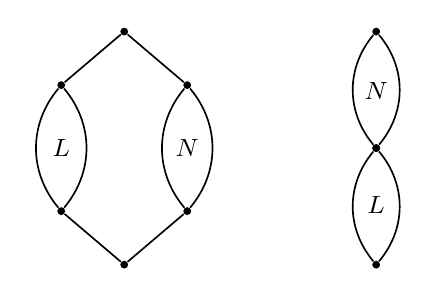
\begin{tikzpicture}[scale=0.4]
    \node (bot) at (0,-3.7) [fill,circle,inner sep=1pt] {};
    \node (top) at (0,3.7) [fill,circle,inner sep=1pt] {};
    \node (botL) at (-2,-2) [fill,circle,inner sep=1pt] {};
    \node (topL) at (-2,2) [fill,circle,inner sep=1pt] {};
    \node (botN) at (2,-2) [fill,circle,inner sep=1pt] {};
    \node (topN) at (2,2) [fill,circle,inner sep=1pt] {};

    \draw[font=\small] (-2,0) node {$L$};
    \draw[font=\small] (2,0) node {$N$};

    \draw[font=\small] (8,-1.8) node {$L$};
    \draw[font=\small] (8,1.8) node {$N$};

    \draw[semithick] 
    (bot) to (botL)
    (bot) to (botN)
    (top) to (topL)
    (top) to (topN);

    \draw [semithick]  
    (botL) to [out=50,in=-50] (topL)
    (botL) to [out=130,in=-130] (topL)
    (botN) to [out=50,in=-50] (topN)
    (botN) to [out=130,in=-130] (topN);

    \node (botLL) at (8,-3.7) [fill,circle,inner sep=1pt] {};
    \node (topLL) at (8,0) [fill,circle,inner sep=1pt] {};
    \node (botNN) at (8,0) [fill,circle,inner sep=1pt] {};
    \node (topNN) at (8,3.7) [fill,circle,inner sep=1pt] {};
    \draw [semithick]  
    (botLL) to [out=50,in=-50] (topLL)
    (botLL) to [out=130,in=-130] (topLL)
    (botNN) to [out=50,in=-50] (topNN)
    (botNN) to [out=130,in=-130] (topNN);
  \end{tikzpicture}
\end{center}
\vspace{0.5em}
}

%%%%%%%%%%%%%%%%%%%%%%%%%%%%%%%%%%%%%%%%%%%%%%%%%%%%%%%%%%%%%%%%%%%%%%%%%%%%%%
\headerbox{References}{name=refs,column=1,span=2,above=bottom}{
% %%%%%%%%%%%%%%%%%%%%%%%%%%%%%%%%%%%%%%%%%%%%%%%%%%%%%%%%%%%%%%%%%%%%%%%%%%%%%%
     \smaller
     \vspace{-0.4em}
     \bibliographystyle{ieee}
     \renewcommand{\section}[2]{\vskip 0.05em}
     \bibliography{wjd}
}
%%%%%%%%%%%%%%%%%%%%%%%%%%%%%%%%%%%%%%%%%%%%%%%%%%%%%%%%%%%%%%%%%%%%%%%%%%%%%%
%   \headerbox{Acknowledgements}{name=funding,column=1,span=2,above=bottom}{
% %%%%%%%%%%%%%%%%%%%%%%%%%%%%%%%%%%%%%%%%%%%%%%%%%%%%%%%%%%%%%%%%%%%%%%%%%%%%%%
%   \smaller 
%   \hspace{1em}This work was supported by the Mathematics Department of the
%   University of \Hawaii\ at \Manoa.
%   }

%%%%%%%%%%%%%%%%%%%%%%%%%%%%%%%%%%%%%%%%%%%%%%%%%%%%%%%%%%%%%%%%%%%%%%%%%%%%%%
  \headerbox{Results}{name=results,column=1,span=2,below=priorwork1 neutralization,above=refs}{
%%%%%%%%%%%%%%%%%%%%%%%%%%%%%%%%%%%%%%%%%%%%%%%%%%%%%%%%%%%%%%%%%%%%%%%%%%%%%%
%      \mbox{\hspace{0.3\linewidth}\rule{0.4\linewidth}{1pt}\hspace{0.3\linewidth}}
%      \hspace{-0.5em}
      \begin{center}
\scalebox{0.44}{\includegraphics{Sevens}}
{\smaller Figure courtesy of Peter Jipsen.}
      \end{center}


%      \mbox{\hspace{0.3\linewidth}\rule{0.4\linewidth}{1pt}\hspace{0.3\linewidth}}
      \begin{multicols}{2}
{\bf Claim:} 
{\it Every lattice with at most 7 elements is
a \mbox{congruence} lattice of a finite algebra.}

\vspace{0.3em}

There are 53 lattices with 7 elements.  We have found representations for all
but these two:

    \begin{center}
  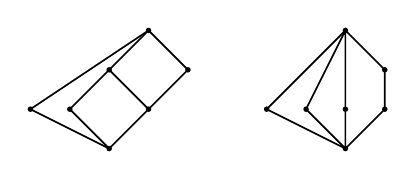
\begin{tikzpicture}[scale=.5]
    % lat5
    \path (-1,1) coordinate (n11); \fill (n11) circle (2pt);
    \path (0,1) coordinate (01); \fill (01) circle (2pt);
    \foreach \j in {0,2} 
    { \path (1,\j) coordinate (1\j); \fill (1\j) circle (2pt); }
    \foreach \j in {1,3} 
    { \path (2,\j) coordinate (2\j); \fill (2\j) circle (2pt); }
    \path (3,2) coordinate (32); \fill (32) circle (2pt);
    \draw[semithick] (10) to (01) to (23) to (32) to (10) (21) to (12);
    \draw[semithick] (10) to (n11) to (23);

    % lat6
    \foreach \j in {0,1,3} 
    { \path (7,\j) coordinate (7\j); \fill (7\j) circle (2pt); }
    \path (6,1) coordinate (61); \fill (61) circle (2pt);
    \path (5,1) coordinate (51); \fill (51) circle (2pt);
    \foreach \j in {1,2} 
    { \path (8,\j) coordinate (8\j); \fill (8\j) circle (2pt); }
    \draw[semithick] (70) to (61) to (73) to (70) to (81) to (82) to (73);
    \draw[semithick] (70) to (51) to (73);
    
  \end{tikzpicture}
\end{center}
\end{multicols}\vspace{-1em}
      \mbox{\hspace{0.3\linewidth}\rule{0.4\linewidth}{1pt}\hspace{0.3\linewidth}}
%\vspace{0.3em}
\begin{center}
{\bf A Galois Correspondence}
\end{center}
For any finite lattice $L$, there is a finite set $A$ such that $L$ can be
embedded into the lattices of all partitions of $A$.  We can
then consider the set $F$ of all operations that respect the partitions of $L$.
If we're lucky, $L$ is the congruence lattice of the resulting algebra \algA.

\vspace{0.5em}

{\bf Nondensity Lemma:} {\it If $L$ is a union of a filter and an ideal, there will
always be nontrivial operations in $F$.}

\mbox{\hspace{0.3\linewidth}\rule{0.4\linewidth}{1pt}\hspace{0.3\linewidth}}

\vspace{-.5em}

\begin{multicols}{2}

    {\bf Gluing Lemma:} {\it Fix two finite congruence lattices $L_1, L_2$ with $\alpha \in
  L_1$ and $\beta \in L_2$.  Under certain conditions, we can prove that the
  following is also a congruence lattice:}
\begin{center}
  
  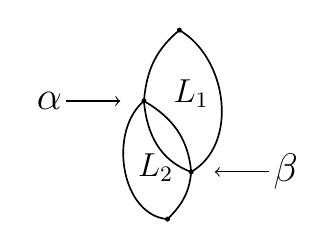
\begin{tikzpicture}[scale=.3]
    % lat5
    \path (0,0) coordinate (bot1); \fill (bot1) circle (3pt);
    \path (-1,5) coordinate (top1); \fill (top1) circle (3pt);
    \path (1,2) coordinate (bot2); \fill (bot2) circle (3pt);
    \path (.5,8) coordinate (top2); \fill (top2) circle (3pt);
    \draw[semithick] 
    (bot1) to [out=45,in=-95] (bot2) to [out=95, in=-30] (top1) to [out=220, in=175] (bot1);
    \draw[semithick] 
    (bot2) to [out=160,in=-85] (top1) to [out=85, in=220] (top2) to [out=-30,
    in=30] (bot2);
    \draw[font=\Large] (-5,5) node {$\alpha$};
    \draw[->] (-4.3,5) -- (-2,5);
    \draw[font=\Large] (5,2) node {$\beta$};
    \draw[->] (4.3,2) -- (2,2);
    \draw[font=\large] (1,5.3) node {$L_1$};
    \draw[font=\large] (-.5,2.2) node {$L_2$};
  \end{tikzpicture}

\end{center}

\end{multicols}
}
%%%%%%%%%%%%%%%%%%%%%%%%%%%%%%%%%%%%%%%%%%%%%%%%%%%%%%%%%%%%%%%%%%%%%%%%%%%%%% 
  \headerbox{Prior Work II}{name=priorwork2,column=2,row=0,above=results,span=1}{
%%%%%%%%%%%%%%%%%%%%%%%%%%%%%%%%%%%%%%%%%%%%%%%%%%%%%%%%%%%%%%%%%%%%%%%%%%%%%%
    \begin{center}
  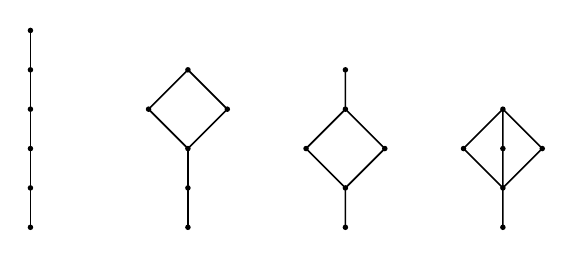
\begin{tikzpicture}[scale=.5]

    % lat1
    \foreach \j in {1,...,6}
    { \path (0,\j) coordinate (0\j); \fill (0\j) circle (2pt); }
    \draw[semithick] (01) to (06);

    % lat2
    \foreach \j in {1,2,3,5}
    { \path (4,\j) coordinate (4\j); \fill (4\j) circle (2pt); }
    \path (3,4) coordinate (34); \fill (34) circle (2pt);
    \path (5,4) coordinate (54); \fill (54) circle (2pt);
    \draw[semithick] (41) to (43) to (34) to (45) to (54) to (43);

    % lat3
    \foreach \j in {1,2,4,5}
    { \path (8,\j) coordinate (8\j); \fill (8\j) circle (2pt); }
    \path (7,3) coordinate (73); \fill (73) circle (2pt);
    \path (9,3) coordinate (93); \fill (93) circle (2pt);
    \draw[semithick] (81) to (82) to (73) to (84) to (85) (84) to (93) to (82);

    % lat4
    \foreach \j in {1,...,4}
    { \path (12,\j) coordinate (12\j); \fill (12\j) circle (2pt); }
    \path (11,3) coordinate (113); \fill (113) circle (2pt);
    \path (13,3) coordinate (133); \fill (133) circle (2pt);
    \draw[semithick] (121) to (124) to (113) to (122) to (133) to (124);
  \end{tikzpicture}
    \end{center}

    \begin{center}
  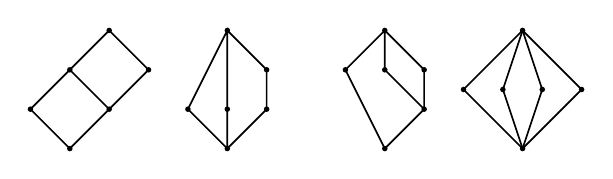
\begin{tikzpicture}[scale=.5]

    % lat5
    \path (0,1) coordinate (01); \fill (01) circle (2pt);
    \foreach \j in {0,2} 
    { \path (1,\j) coordinate (1\j); \fill (1\j) circle (2pt); }
    \foreach \j in {1,3} 
    { \path (2,\j) coordinate (2\j); \fill (2\j) circle (2pt); }
    \path (3,2) coordinate (32); \fill (32) circle (2pt);
    \draw[semithick] (10) to (01) to (23) to (32) to (10) (21) to (12);

    % lat6
    \foreach \j in {0,1,3} 
    { \path (5,\j) coordinate (5\j); \fill (5\j) circle (2pt); }
    \path (4,1) coordinate (41); \fill (41) circle (2pt);
    \foreach \j in {1,2} 
    { \path (6,\j) coordinate (6\j); \fill (6\j) circle (2pt); }
    \draw[semithick] (50) to (41) to (53) to (50) to (61) to (62) to (53);
    
    % lat7
%    \foreach \i in {7,8,9} 
    \foreach \i in {8,9,10} 
    { \path (\i,2) coordinate (\i2); \fill (\i2) circle (2pt); }
    \path (9,0) coordinate (90); \fill (90) circle (2pt);
    \path (9,3) coordinate (93); \fill (93) circle (2pt);
    \path (10,1) coordinate (101); \fill (101) circle (2pt);
    \draw[semithick] (90) to (82) to (93) to (92) to (101) to (90) (101) to (102) to (93);

    % lat8
    \foreach \j in {0,3}
    { 
      \path (12.5,\j) coordinate (125\j); 
      \fill (125\j) circle (2pt);
    }
    \foreach \i in {11,...,14}
    { 
      \path (\i,1.5) coordinate (\i15); 
      \fill (\i15) circle (2pt);
      \draw[semithick] (\i15) to (1250);
      \draw[semithick] (\i15) to (1253);
    }

  \end{tikzpicture}
    \end{center}

    \begin{center}
  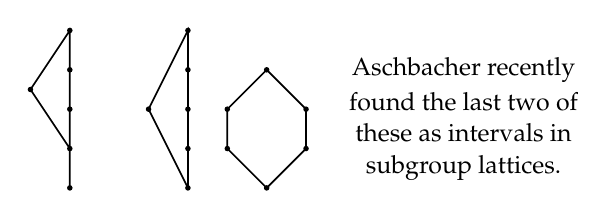
\begin{tikzpicture}[scale=.5]

    % lat9
    \foreach \j in {1,...,5}
    { \path (1,\j) coordinate (1\j); \fill (1\j) circle (2pt); }
    \path (0,3.5) coordinate (035); \fill (035) circle (2pt);
    \draw[semithick] (11) to (15) to (035) to (12);

    % lat10
    \foreach \j in {1,...,5}
    { \path (4,\j) coordinate (4\j); \fill (4\j) circle (2pt); }
    \path (3,3) coordinate (33); \fill (33) circle (2pt);
    \draw[semithick] (41) to (45) to (33) to (41);

    % lat11
    \foreach \j in {2,3}
    { \path (5,\j) coordinate (5\j); \fill (5\j) circle (2pt);
      \path (7,\j) coordinate (7\j); \fill (7\j) circle (2pt); }
    \foreach \j in {1,4} 
    { \path (6,\j) coordinate (6\j); \fill (6\j) circle (2pt);}
    \draw[semithick] (61) to (52) to (53) to (64) to (73) to (72) to (61);

    \draw[font=\small] (11,4) node {Aschbacher recently};
    \draw[font=\small] (11,3.2) node {found the last two of};
    \draw[font=\small] (11,2.4) node {these as intervals in};
    \draw[font=\small] (11,1.5) node {subgroup lattices.};
    
  \end{tikzpicture}
    \end{center}

{\bf Theorem:} {\it Every lattice with at most 6 elements is
a \mbox{congruence} lattice of a finite algebra.}
}



%     \smaller
%     \vspace{-0.4em}
%     \bibliographystyle{ieee}
%     \renewcommand{\section}[2]{\vskip 0.05em}
%       \begin{thebibliography}{1}\itemsep=-0.01em
%       \setlength{\baselineskip}{0.4em}
%       \bibitem{amberg07:nonrigid}
%         B.~Amberg, S.~Romdhani, T. Vetter.
%         \newblock {O}ptimal {S}tep {N}onrigid {ICP} {A}lgorithms for {S}urface {R}egistration
%         \newblock In {\em Computer Vision and Pattern Recognition 2007}
%       \bibitem{amberg08:recognition}
%         B.~Amberg, R.~Knothe, T. Vetter.
%         \newblock Expression Invariant Face Recognition with a 3D Morphable Model
%         \newblock In {\em Automated Face and Gesture Recognition 2008}
%       \end{thebibliography}
%   }

%%%%%%%%%%%%%%%%%%%%%%%%%%%%%%%%%%%%%%%%%%%%%%%%%%%%%%%%%%%%%%%%%%%%%%%%%%%%%%
  \headerbox{Decompositions of algebras}{name=decomp,column=0,span=1,above=bottom}{
%%%%%%%%%%%%%%%%%%%%%%%%%%%%%%%%%%%%%%%%%%%%%%%%%%%%%%%%%%%%%%%%%%%%%%%%%%%%%%
\vspace{.3em}

\begin{center}
    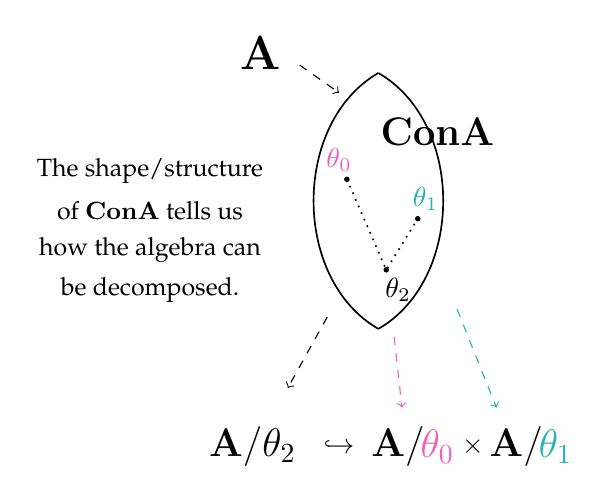
\begin{tikzpicture}[scale=.5]
      \draw[font=\LARGE] (-3,7) node {$\bA$};
      \draw[->,dashed] (-2,6.7) -- (-1,6);
      \draw[->,dashed] (-1.3,.3) -- (-2.3,-1.5);
%      \draw[->,dashed,Orange] (.4,-.2) -- (.6,-2);
%      \draw[->,dashed,red] (.4,-.2) -- (.6,-2);
      \draw[->,dashed,CarnationPink] (.4,-.2) -- (.6,-2);
      \draw[->,dashed,TealBlue] (2,.5) -- (3,-2);
%      \draw[->,dashed,Green] (2,.5) -- (3,-2);
      \draw[font=\Large] (1.5,5) node {$\bCon \bA$};
\draw[font=\small] (-5.8,4) node {The shape/structure};
\draw[font=\small] (-5.8,3) node {of $\bCon \bA$ tells us};
\draw[font=\small] (-5.8,2) node {how the algebra can};
\draw[font=\small] (-5.8,1) node {be decomposed.};

      \draw[semithick] (0,6.5) to [out=210,in=150] (0,0);% \fill (0,0) circle (2pt);
      \draw[semithick] (0,0) to [out=30,in=-30] (0,6.5);% \fill (0,6.5) circle (2pt);
%            \draw[Orange] (-1,4.3) node {$\theta_0$};
            \draw[CarnationPink] (-1,4.3) node {$\theta_0$};
%            \draw[red] (-1,4.3) node {$\theta_0$};
      \draw[TealBlue] (1.2,3.3) node {$\theta_1$};
%      \draw[Green] (1.2,3.3) node {$\theta_1$};
      \draw (.5,1) node {$\theta_2$};
      \draw[semithick, dotted] (-.8,3.8) to (.2,1.5) to (1,2.8);
      \fill (-.8,3.8) circle (2pt); 
      \fill (.2,1.5) circle (2pt); 
      \fill (1,2.8) circle (2pt); 

      \draw[font=\Large] (-3.2,-3) node {$\bA/\theta_2$}; 
%      \draw[font=\large] (-1,-3) node {$\hookrightarrow$};
      \draw (-1,-3) node {$\hookrightarrow$};
      \draw[font=\Large] (.5,-3) node {$\bA/$};
      \draw[font=\Large,CarnationPink] (1.5,-3) node {$\theta_0$};
%      \draw[font=\Large,Orange] (1.5,-3) node {$\theta_0$};
%      \draw[font=\Large,red] (1.5,-3) node {$\theta_0$};
%      \draw[font=\large] (2.5,-3) node {$\times$};
      \draw (2.4,-3) node {$\times$};
      \draw[font=\Large] (3.5,-3) node {$\bA/$};
      \draw[font=\Large,TealBlue] (4.5,-3) node {$\theta_1$};
%      \draw[font=\Large,Green] (4.5,-3) node {$\theta_1$};
%      \draw[font=\Large] (0,-3) node {$\bA/\theta_2 \hookrightarrow \bA/\theta_0 \times \bA/\theta_1$};
%      \path[->] (1.8,3.3) edge node[above] {$F$} (4.5,3.3);
    \end{tikzpicture}
  \end{center}

\vspace{.3em}

}

%%%%%%%%%%%%%%%%%%%%%%%%%%%%%%%%%%%%%%%%%%%%%%%%%%%%%%%%%%%%%%%%%%%%%%%%%%%%%%
  \headerbox{The basic structure of an algebra}{name=structure,column=0,span=1,below=algebra,above=decomp}{
%%%%%%%%%%%%%%%%%%%%%%%%%%%%%%%%%%%%%%%%%%%%%%%%%%%%%%%%%%%%%%%%%%%%%%%%%%%%%%
{}A {\bf congruence} of an algebra $\bA = \algA$ is a partition of the set $A$
into blocks that are preserved by the operations in $F$.

    \begin{center}
    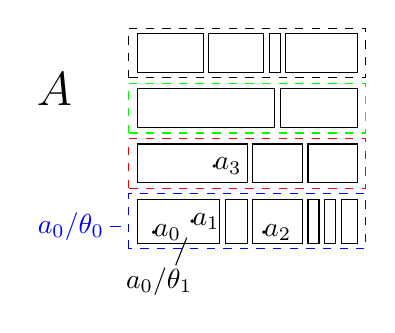
\begin{tikzpicture}[scale=.7]
      \draw[dashed,blue] (-.15,0.1) rectangle (4.15,1.1);
      \draw[dashed,red] (-.15,1.2) rectangle (4.15,2.1);
      \draw[dashed,green] (-.15,2.2) rectangle (4.15,3.1);
      \draw[dashed] (-.15,3.2) rectangle (4.15,4.1);

      \draw (0,0.2) rectangle (1.5,1)
      (1.6,0.2) rectangle (2,1)
      (2.1,0.2) rectangle (3,1)
      (3.1,0.2) rectangle (3.3,1)
      (3.4,0.2) rectangle (3.6,1)
      (3.7,0.2) rectangle (4,1);
      \fill (.3,.4) circle (1pt);
      \draw (.55,.4) node {$a_0$};
      \fill (1,.6) circle (1pt);
      \draw (1.25,.6) node {$a_1$};
      \fill (2.3,.4) circle (1pt);
      \draw (2.55,.4) node {$a_2$};

      \draw[font=\LARGE] (-1.5,3) node {$A$};

      \draw (0,1.3) rectangle (2,2)
      (2.1,1.3) rectangle (3,2)
      (3.1,1.3) rectangle (4,2);
      \fill (1.4,1.6) circle (1pt);
      \draw (1.65,1.6) node {$a_3$};

      \draw[blue] (-1.2,.5) node {$a_0/\theta_0$};
      \draw[blue] (-.5,.5) -- (-.3,.5);
      \draw (.4,-.5) node {$a_0/\theta_1$};
      \draw (.7,-.2) -- (.9,.3);

      \draw (0,2.3) rectangle (2.5,3)
      (2.6,2.3) rectangle (4,3);

      \draw (0,3.3) rectangle (1.2,4)
      (1.3,3.3) rectangle (2.3,4)
      (2.4,3.3) rectangle (2.6,4)
      (2.7,3.3) rectangle (4,4);
      % \fill (3.3,3.4) circle (1pt);
      % \draw (3.55,3.4) node {$a_4$};
    \end{tikzpicture}
    \end{center}
The set of all congruences of an algebra forms the {\bf congruence lattice} of
the algebra, denoted $\bCon \bA$. 
Insight into the structure of $\bA$ is gained by knowing the shape of
$\bCon \bA$. 
\vspace{-0.3em}
}


\end{poster}

\end{document}
